\documentclass[12pt]{article}
\title{Mapping rainfall anomalies during the 2015-2016 El Ni{\~n}o event}
\author{P. Krishna Krishnamurthy | UCLA ID: 904723392}
\date{}
\usepackage{graphicx}
\usepackage{float}
\usepackage{textcomp}
\usepackage{listings}
\usepackage{subfig}

\begin{document}
\maketitle

\begin{abstract}
There is consensus in the climate science community that El Ni{\~n}o events, periods of anomalously high sea surface temperatures in the Pacific, are associated with disruptions to monsoon patterns which lead to changes in rainfall patterns. The 2015-2016 El Ni{\~n}o episode was an unprecedented event of a scale not seen before, and there is concern that such events may become more frequent under climate change. Understanding rainfall anomalies associated with such large-scale events is the first step towards anticipating potential impacts on vulnerable systems including rain-fed agriculture. Here I utilize remotely-sensed data from the Tropical Rainfall Measurement Mission (TRMM) and the Global Precipitation Measurement Mission (GPM) to illustrate the geographic distributions of rainfall anomalies reported in 2016, at the peak of the recent 2014-2016 Ni{\~n}o event.
\end{abstract}

\section{Introduction}
El Ni{\~n}o events, periods of anomalously high sea surface temperatures in the Pacific, are associated with disruptions to monsoon patterns which lead to changes in rainfall patterns. The 2014-2016 El Ni{\~n}o episode was an unprecedented event of a scale not seen before, and there is concern that such events may become more frequent under climate change \cite{cai2014increasing}. Understanding rainfall anomalies associated with such large-scale events is the first step towards anticipating potential impacts on vulnerable systems including rain-fed agriculture. This information can then be used to understand which societies or systems are particularly vulnerable to strong El Ni{\~n}o episodes, and can be used to prepare risk management strategies \cite{wang2017nino}. 

\section{Materials \& Methods}
\subsection{Data}
The TRMM satellite was launched in November 1997 and terminated operations in April 2015. The satellite provided rainfall information at a high spatial resolution (1 degree  by 1 degree) and very high temporal resolution (every 3 hours) for all coordinates between 50\textdegree N and 50\textdegree S. The GPM was launched in February 2014 building on the successes of TRMM and provides compatibility with TRMM datasets. The main difference between the two datasets is that GPM provides data for coordinates between 60\textdegree N and 60\textdegree S. For comparability, results are shown for all coordinates between 50\textdegree N and 50\textdegree S. Data are available for download in 3-hour, 1-day, and 30-day intervals.

Monthly average rainfall rates (measured in terms of mm/hr) were downloaded for the period 1998-2014 from the NASA-TRMM server, and for the period 2015-2016 from the NASA-GPM server. To determine historical rainfall climatology, the average rainfall rate was calculated for the period 1998-2015. A thirty-year dataset is usually considered to be sufficient to establish climatology; unfortunately the historical data are limited so climatology is established using data over a 17-year period. To determine rainfall anomalies in 2016, the difference between the average rainfall values of 2016 and the 17-year historical average was calculated.

However, annual rainfall anomalies only tell part of the story. To better understand the impact of El Ni{\~n}o episodes, it is useful to also consider seasonal rainfall patterns. Seasons were defined as follows: boreal winter (December, January, February), boreal spring (March, April, May), boreal summer (June, July, August), and boreal autumn (September, October, November) following convention in climate science cf. \cite{larkin2005global}. Seasonal anomalies were calculated by first calculating seasonal averages between December 2015 and November 2016, and comparing those to seasonal average rainfall rates between December 1997 and November 2015 (the latter is again considered climatology).      
 
\subsection{Annotated code}
Here I will add all codes used for the project.

Here is the first code I used for this project. The function takes in an HDF file, a title and destination path, and generates a map using the title and path specified by the user:\\

\lstset{language=Python, basicstyle=\footnotesize\ttfamily}  
\begin{lstlisting}[frame=single]
# import libraries and modules
from mpl_toolkits.basemap import Basemap, cm
import matplotlib.pyplot as plt
import matplotlib.image as mpimg
import numpy as np
import h5py as h5py

def mapplot(filename, title_name, fig_path):
    #this function maps the results of a HDF5 file. 
    #the function takes three arguments 
    #(the path to the filename, 
    #the desired title for the image, 
    #and the path to where the plot should be saved)

    dataset = h5py.File(filename, 'r') 
    
    # Get precipitation data only
    precip = dataset['Grid/precipitation'][:]
    precip = np.transpose(precip)

    # Get longitudes and latitudes
    theLats = dataset['Grid/lat'][:]
    theLons = dataset['Grid/lon'][:]

    # Plot the figure, define the geographic bounds
    fig = plt.figure(dpi=300)
    latcorners = ([-60,60])
    loncorners = ([-180,180])

    m = Basemap(projection='cyl',llcrnrlat=latcorners[0],\
	urcrnrlat=latcorners[1],llcrnrlon=loncorners[0],\
	urcrnrlon=loncorners[1])

    # Draw coastlinescountry boundaries, edge of map.
    m.drawcoastlines()
    # m.drawstates() # no need for states for this map
    m.drawcountries()

    # Draw filled contours.
    clevs = np.arange(0,1.26,0.125)

    # Define the latitude and longitude data
    x, y = np.float32(np.meshgrid(theLons, theLats))

    # Mask the values less than 0.
    masked_array = np.ma.masked_where(precip < 0,precip) 

    # Assign color scheme
    cmap = cm.GMT_drywet

    # Plot the data
    cs = m.contourf(x,y,precip,clevs,cmap=cmap,latlon=True) 
	# reports error due to deprecation but produces map
    parallels = np.arange(-60.,61,20.)
    m.drawparallels(parallels,labels=[True,False,True,False])
    meridians = np.arange(-180.,180.,60.)
    m.drawmeridians(meridians,labels=[False,False,False,True])

    #Set the title and fonts
    plt.title(title_name)
    font = {'weight' : 'bold', 'size' : 6}
    plt.rc('font', **font)

    #Add colorbar
    cbar = m.colorbar(cs,location='right',pad="5%")
    cbar.set_label('mm/h')
    #Save figure in desired path
    plt.savefig(fig_path,dpi=200) 

\end{lstlisting}

\section{Results}
\textbf{Note: This section will be expanded for the final draft of the report.}\\

Figure 1 below shows mean monthly rainfall rates in 2016 and in the period 1998-2015 (considered the baseline in this analysis).

\begin{figure}[htb]
    \label{fig:averages}
\centering
  \subfloat[Mean monthly rainfall rates (2016)]{%
    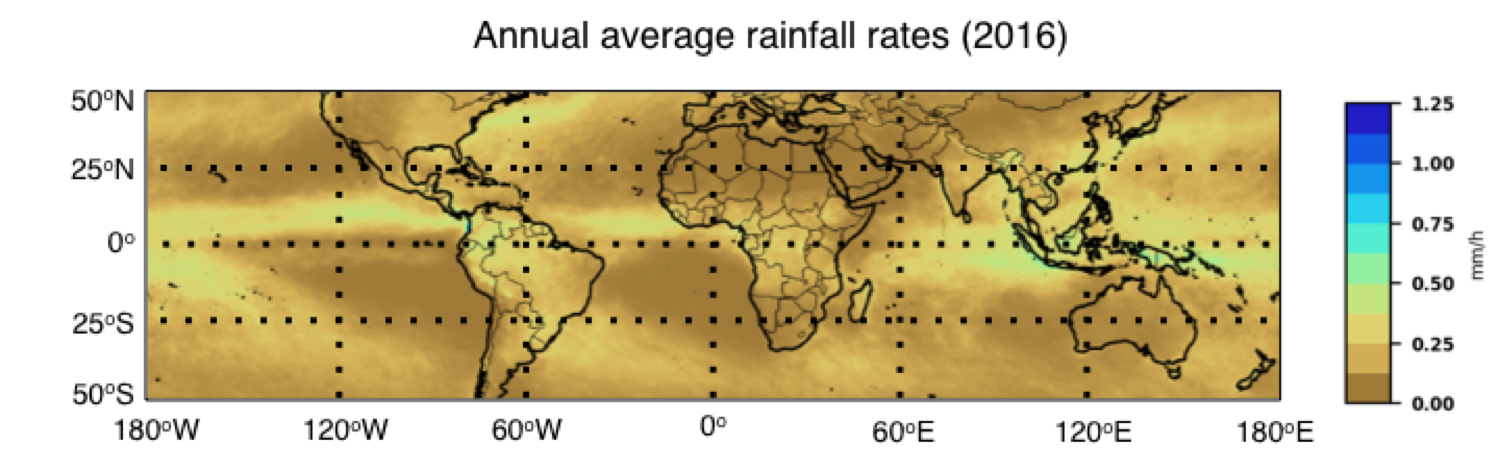
\includegraphics[width=1\textwidth]{figures/2016-ave.png}}\hfill
  \subfloat[Mean monthly rainfall rates (historical average)]{%
    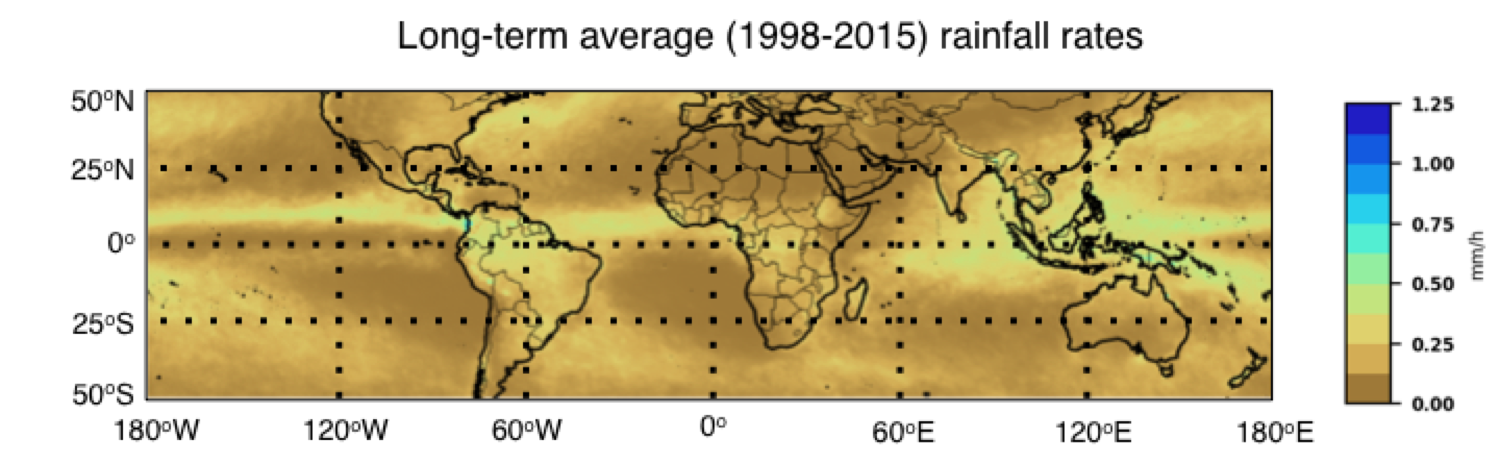
\includegraphics[width=1\textwidth]{figures/lta-ave.png}}\hfill
\caption{Mean monthly rainfall rates for 2016 and the historical average (1998-2015)}
\end{figure}

While the two plots are largely similar, there are discernible differences between the two: the western parts of the Indonesian archipelago appear to have received more rainfall than the mainland areas, and the Philippine Islands received substantially lower rainfall in 2016 than in the historical average.

In order to better assess rainfall anomalies, it is useful to consider the differences in rainfall values between 2016 and the historical average (Figure 2). The plot highlights significant rainfall deficiencies in large parts of Indonesia, the Philippines and parts of Sri Lanka. Such anomalies have broader social implications as these countries are major rice producers and exporters; given that paddy production requires significant amounts of water and that irrigation is limited in these countries, reductions in rainfall can result in reduced rice production with food security implications at the national, regional and global levels \cite{zubair2002nino, haile2005weather}. 

\begin{figure}[H]
    \label{fig:lta-difference}
\begin{center}
   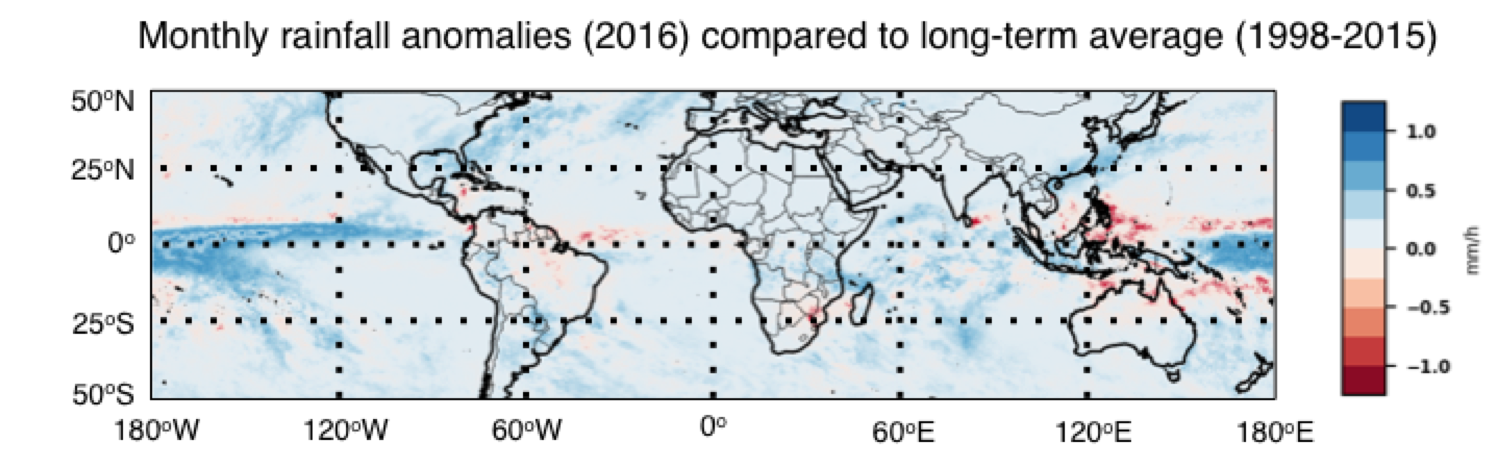
\includegraphics[width=1.15\linewidth]{figures/lta-diff.png}
\end{center}
\caption{Average monthly rainfall anomalies in 2016 compared to the historical average (1998-2015)}
\end{figure}

However, rainfall anomalies on their own are not enough to cause a food security crisis. Reductions in rainfall during the key growing season are what cause major crop production deficits. It is therefore useful to consider seasonal rainfall anomalies (Figure 3). As shown below, rainfall levels during the period December-February were significantly below the historical average. 

\begin{figure}[H]
    \label{fig:seasonal-anomalies}
\centering
  \subfloat[Seasonal rainfall anomalies (DJF)]{%
    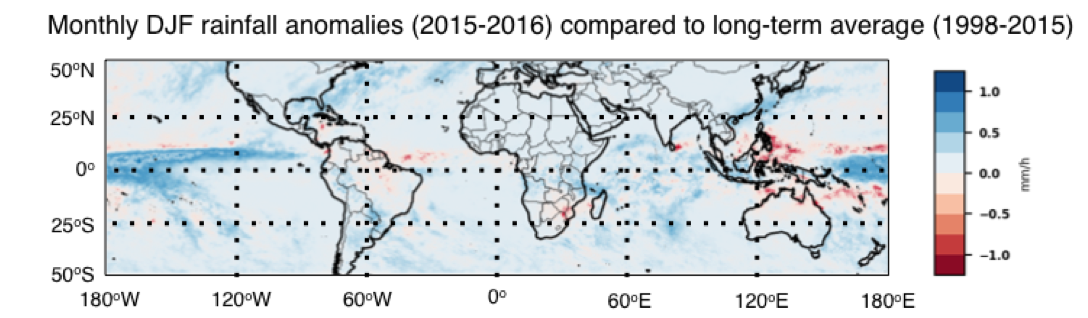
\includegraphics[width=.65\linewidth]{figures/djf-diff.png}}\hfill
  \subfloat[Seasonal rainfall anomalies (MAM)]{%
    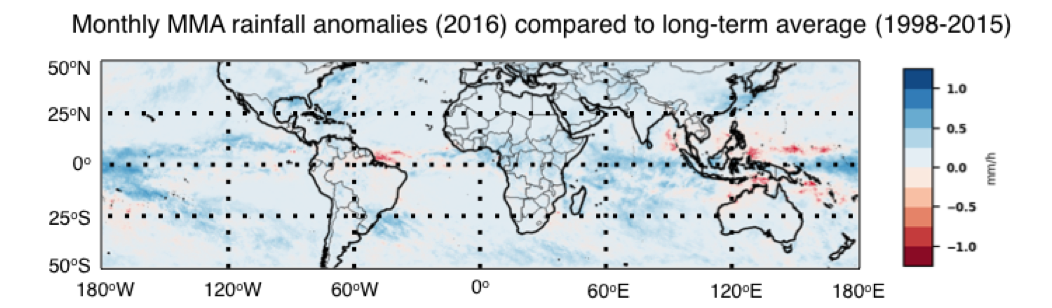
\includegraphics[width=.65\linewidth]{figures/mam-diff.png}}\hfill
  \subfloat[Seasonal rainfall anomalies (JJA)]{%
    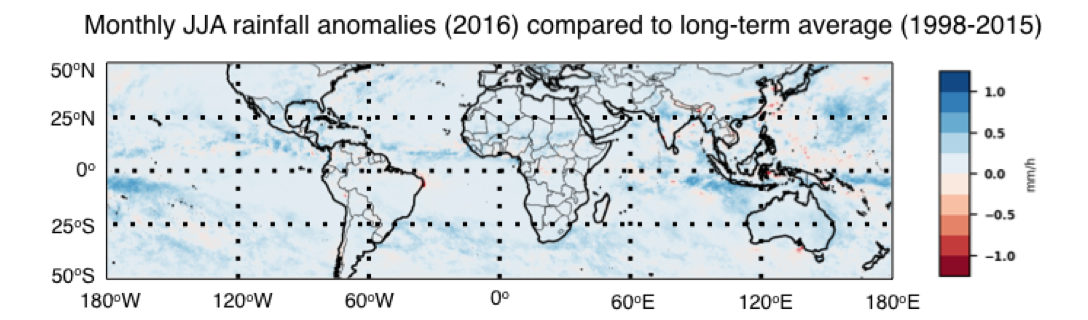
\includegraphics[width=.65\linewidth]{figures/jja-diff.png}}\hfill  
  \subfloat[Seasonal rainfall anomalies (SON)]{%
    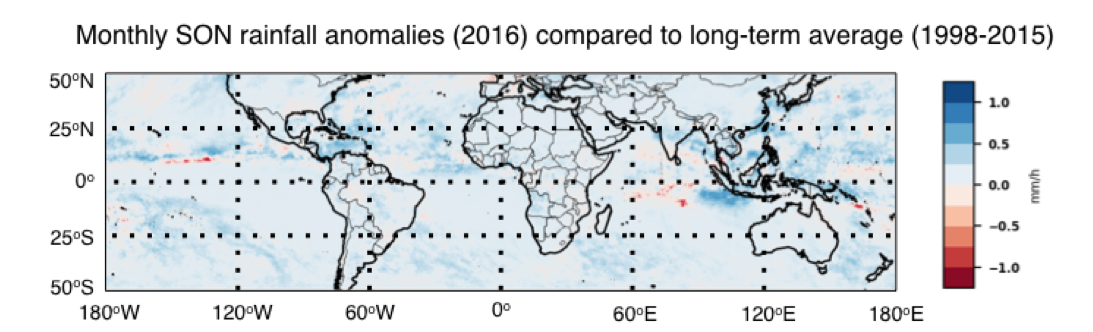
\includegraphics[width=.65\linewidth]{figures/son-diff.png}}\hfill
\caption{Seasonal rainfall anomalies}
\end{figure}

In the Indonesian archipelago, the key agricultural season occurs between December and February. Reductions in rainfall can therefore have significant impacts on national agricultural production \cite{naylor2001using}. In the Philippines, a minor growing season occurs in this period. Paddy produced in this minor rainy season is normally exported; given that rice exports contribute significantly to the Philippine economy, lower rice production associated with Ni{\~n}o can have major deleterious economic consequences.

\bibliography{eeb177.bib}
\bibliographystyle{apalike}

\end{document}
